\documentclass{article}
\usepackage{amsmath}
\usepackage{listings}
\usepackage{enumitem,kantlipsum}

% ============================================================
% INFR11269 Machine Learning Systems — Coursework Report
% Academic year 2026/27
%
% This coursework uses the official ICLR 2027 LaTeX style.
%
% IMPORTANT FORMAT RULES
% - Do not edit iclr2027_conference.sty.
% - Do not change page geometry, text width/height, base font size,
%   or line spacing.
% - Do not enable \iclrfinalcopy.
% - Normal content packages are fine if they do not alter the report format.
%
% Main-body page limit: six pages.
% References and Appendix do NOT count toward the main-body page limit.
% Reviewers are not obliged to read Appendix at all. Please put your main content
% in the main body.
% 
% AI policy:
% Academic integrity is an underlying principle of research and academic practice.
% All submitted work is expected to be your own, including any material you have
% generated yourself with the assistance of AI tools such as ELM, ChatGPT,
% Bing Chat, Claude, Google Gemini, or any other automated assistance.
% For all such material you must make prominent explicit acknowledgement and
% explain clearly what you have done in the AI declaration section.
% This includes using AI to directly generate text, code, figures or similar
% or to complete other tasks. In all cases, you remain entirely responsible
% for the material you produce.
% ============================================================

\usepackage{iclr2027_conference,times}

\usepackage{hyperref}
\usepackage{url}
\usepackage{booktabs}
\usepackage{graphicx}
\usepackage{amsmath}
\usepackage{amssymb}

% The official ICLR archive includes math_commands.tex. It is optional:
%%%%% NEW MATH DEFINITIONS %%%%%

\usepackage{amsmath,amsfonts,bm}

% Mark sections of captions for referring to divisions of figures
\newcommand{\figleft}{{\em (Left)}}
\newcommand{\figcenter}{{\em (Center)}}
\newcommand{\figright}{{\em (Right)}}
\newcommand{\figtop}{{\em (Top)}}
\newcommand{\figbottom}{{\em (Bottom)}}
\newcommand{\captiona}{{\em (a)}}
\newcommand{\captionb}{{\em (b)}}
\newcommand{\captionc}{{\em (c)}}
\newcommand{\captiond}{{\em (d)}}

% Highlight a newly defined term
\newcommand{\newterm}[1]{{\bf #1}}


% Figure reference, lower-case.
\def\figref#1{figure~\ref{#1}}
% Figure reference, capital. For start of sentence
\def\Figref#1{Figure~\ref{#1}}
\def\twofigref#1#2{figures \ref{#1} and \ref{#2}}
\def\quadfigref#1#2#3#4{figures \ref{#1}, \ref{#2}, \ref{#3} and \ref{#4}}
% Section reference, lower-case.
\def\secref#1{section~\ref{#1}}
% Section reference, capital.
\def\Secref#1{Section~\ref{#1}}
% Reference to two sections.
\def\twosecrefs#1#2{sections \ref{#1} and \ref{#2}}
% Reference to three sections.
\def\secrefs#1#2#3{sections \ref{#1}, \ref{#2} and \ref{#3}}
% Reference to an equation, lower-case.
\def\eqref#1{equation~\ref{#1}}
% Reference to an equation, upper case
\def\Eqref#1{Equation~\ref{#1}}
% A raw reference to an equation---avoid using if possible
\def\plaineqref#1{\ref{#1}}
% Reference to a chapter, lower-case.
\def\chapref#1{chapter~\ref{#1}}
% Reference to an equation, upper case.
\def\Chapref#1{Chapter~\ref{#1}}
% Reference to a range of chapters
\def\rangechapref#1#2{chapters\ref{#1}--\ref{#2}}
% Reference to an algorithm, lower-case.
\def\algref#1{algorithm~\ref{#1}}
% Reference to an algorithm, upper case.
\def\Algref#1{Algorithm~\ref{#1}}
\def\twoalgref#1#2{algorithms \ref{#1} and \ref{#2}}
\def\Twoalgref#1#2{Algorithms \ref{#1} and \ref{#2}}
% Reference to a part, lower case
\def\partref#1{part~\ref{#1}}
% Reference to a part, upper case
\def\Partref#1{Part~\ref{#1}}
\def\twopartref#1#2{parts \ref{#1} and \ref{#2}}

\def\ceil#1{\lceil #1 \rceil}
\def\floor#1{\lfloor #1 \rfloor}
\def\1{\bm{1}}
\newcommand{\train}{\mathcal{D}}
\newcommand{\valid}{\mathcal{D_{\mathrm{valid}}}}
\newcommand{\test}{\mathcal{D_{\mathrm{test}}}}

\def\eps{{\epsilon}}


% Random variables
\def\reta{{\textnormal{$\eta$}}}
\def\ra{{\textnormal{a}}}
\def\rb{{\textnormal{b}}}
\def\rc{{\textnormal{c}}}
\def\rd{{\textnormal{d}}}
\def\re{{\textnormal{e}}}
\def\rf{{\textnormal{f}}}
\def\rg{{\textnormal{g}}}
\def\rh{{\textnormal{h}}}
\def\ri{{\textnormal{i}}}
\def\rj{{\textnormal{j}}}
\def\rk{{\textnormal{k}}}
\def\rl{{\textnormal{l}}}
% rm is already a command, just don't name any random variables m
\def\rn{{\textnormal{n}}}
\def\ro{{\textnormal{o}}}
\def\rp{{\textnormal{p}}}
\def\rq{{\textnormal{q}}}
\def\rr{{\textnormal{r}}}
\def\rs{{\textnormal{s}}}
\def\rt{{\textnormal{t}}}
\def\ru{{\textnormal{u}}}
\def\rv{{\textnormal{v}}}
\def\rw{{\textnormal{w}}}
\def\rx{{\textnormal{x}}}
\def\ry{{\textnormal{y}}}
\def\rz{{\textnormal{z}}}

% Random vectors
\def\rvepsilon{{\mathbf{\epsilon}}}
\def\rvtheta{{\mathbf{\theta}}}
\def\rva{{\mathbf{a}}}
\def\rvb{{\mathbf{b}}}
\def\rvc{{\mathbf{c}}}
\def\rvd{{\mathbf{d}}}
\def\rve{{\mathbf{e}}}
\def\rvf{{\mathbf{f}}}
\def\rvg{{\mathbf{g}}}
\def\rvh{{\mathbf{h}}}
\def\rvu{{\mathbf{i}}}
\def\rvj{{\mathbf{j}}}
\def\rvk{{\mathbf{k}}}
\def\rvl{{\mathbf{l}}}
\def\rvm{{\mathbf{m}}}
\def\rvn{{\mathbf{n}}}
\def\rvo{{\mathbf{o}}}
\def\rvp{{\mathbf{p}}}
\def\rvq{{\mathbf{q}}}
\def\rvr{{\mathbf{r}}}
\def\rvs{{\mathbf{s}}}
\def\rvt{{\mathbf{t}}}
\def\rvu{{\mathbf{u}}}
\def\rvv{{\mathbf{v}}}
\def\rvw{{\mathbf{w}}}
\def\rvx{{\mathbf{x}}}
\def\rvy{{\mathbf{y}}}
\def\rvz{{\mathbf{z}}}

% Elements of random vectors
\def\erva{{\textnormal{a}}}
\def\ervb{{\textnormal{b}}}
\def\ervc{{\textnormal{c}}}
\def\ervd{{\textnormal{d}}}
\def\erve{{\textnormal{e}}}
\def\ervf{{\textnormal{f}}}
\def\ervg{{\textnormal{g}}}
\def\ervh{{\textnormal{h}}}
\def\ervi{{\textnormal{i}}}
\def\ervj{{\textnormal{j}}}
\def\ervk{{\textnormal{k}}}
\def\ervl{{\textnormal{l}}}
\def\ervm{{\textnormal{m}}}
\def\ervn{{\textnormal{n}}}
\def\ervo{{\textnormal{o}}}
\def\ervp{{\textnormal{p}}}
\def\ervq{{\textnormal{q}}}
\def\ervr{{\textnormal{r}}}
\def\ervs{{\textnormal{s}}}
\def\ervt{{\textnormal{t}}}
\def\ervu{{\textnormal{u}}}
\def\ervv{{\textnormal{v}}}
\def\ervw{{\textnormal{w}}}
\def\ervx{{\textnormal{x}}}
\def\ervy{{\textnormal{y}}}
\def\ervz{{\textnormal{z}}}

% Random matrices
\def\rmA{{\mathbf{A}}}
\def\rmB{{\mathbf{B}}}
\def\rmC{{\mathbf{C}}}
\def\rmD{{\mathbf{D}}}
\def\rmE{{\mathbf{E}}}
\def\rmF{{\mathbf{F}}}
\def\rmG{{\mathbf{G}}}
\def\rmH{{\mathbf{H}}}
\def\rmI{{\mathbf{I}}}
\def\rmJ{{\mathbf{J}}}
\def\rmK{{\mathbf{K}}}
\def\rmL{{\mathbf{L}}}
\def\rmM{{\mathbf{M}}}
\def\rmN{{\mathbf{N}}}
\def\rmO{{\mathbf{O}}}
\def\rmP{{\mathbf{P}}}
\def\rmQ{{\mathbf{Q}}}
\def\rmR{{\mathbf{R}}}
\def\rmS{{\mathbf{S}}}
\def\rmT{{\mathbf{T}}}
\def\rmU{{\mathbf{U}}}
\def\rmV{{\mathbf{V}}}
\def\rmW{{\mathbf{W}}}
\def\rmX{{\mathbf{X}}}
\def\rmY{{\mathbf{Y}}}
\def\rmZ{{\mathbf{Z}}}

% Elements of random matrices
\def\ermA{{\textnormal{A}}}
\def\ermB{{\textnormal{B}}}
\def\ermC{{\textnormal{C}}}
\def\ermD{{\textnormal{D}}}
\def\ermE{{\textnormal{E}}}
\def\ermF{{\textnormal{F}}}
\def\ermG{{\textnormal{G}}}
\def\ermH{{\textnormal{H}}}
\def\ermI{{\textnormal{I}}}
\def\ermJ{{\textnormal{J}}}
\def\ermK{{\textnormal{K}}}
\def\ermL{{\textnormal{L}}}
\def\ermM{{\textnormal{M}}}
\def\ermN{{\textnormal{N}}}
\def\ermO{{\textnormal{O}}}
\def\ermP{{\textnormal{P}}}
\def\ermQ{{\textnormal{Q}}}
\def\ermR{{\textnormal{R}}}
\def\ermS{{\textnormal{S}}}
\def\ermT{{\textnormal{T}}}
\def\ermU{{\textnormal{U}}}
\def\ermV{{\textnormal{V}}}
\def\ermW{{\textnormal{W}}}
\def\ermX{{\textnormal{X}}}
\def\ermY{{\textnormal{Y}}}
\def\ermZ{{\textnormal{Z}}}

% Vectors
\def\vzero{{\bm{0}}}
\def\vone{{\bm{1}}}
\def\vmu{{\bm{\mu}}}
\def\vtheta{{\bm{\theta}}}
\def\va{{\bm{a}}}
\def\vb{{\bm{b}}}
\def\vc{{\bm{c}}}
\def\vd{{\bm{d}}}
\def\ve{{\bm{e}}}
\def\vf{{\bm{f}}}
\def\vg{{\bm{g}}}
\def\vh{{\bm{h}}}
\def\vi{{\bm{i}}}
\def\vj{{\bm{j}}}
\def\vk{{\bm{k}}}
\def\vl{{\bm{l}}}
\def\vm{{\bm{m}}}
\def\vn{{\bm{n}}}
\def\vo{{\bm{o}}}
\def\vp{{\bm{p}}}
\def\vq{{\bm{q}}}
\def\vr{{\bm{r}}}
\def\vs{{\bm{s}}}
\def\vt{{\bm{t}}}
\def\vu{{\bm{u}}}
\def\vv{{\bm{v}}}
\def\vw{{\bm{w}}}
\def\vx{{\bm{x}}}
\def\vy{{\bm{y}}}
\def\vz{{\bm{z}}}

% Elements of vectors
\def\evalpha{{\alpha}}
\def\evbeta{{\beta}}
\def\evepsilon{{\epsilon}}
\def\evlambda{{\lambda}}
\def\evomega{{\omega}}
\def\evmu{{\mu}}
\def\evpsi{{\psi}}
\def\evsigma{{\sigma}}
\def\evtheta{{\theta}}
\def\eva{{a}}
\def\evb{{b}}
\def\evc{{c}}
\def\evd{{d}}
\def\eve{{e}}
\def\evf{{f}}
\def\evg{{g}}
\def\evh{{h}}
\def\evi{{i}}
\def\evj{{j}}
\def\evk{{k}}
\def\evl{{l}}
\def\evm{{m}}
\def\evn{{n}}
\def\evo{{o}}
\def\evp{{p}}
\def\evq{{q}}
\def\evr{{r}}
\def\evs{{s}}
\def\evt{{t}}
\def\evu{{u}}
\def\evv{{v}}
\def\evw{{w}}
\def\evx{{x}}
\def\evy{{y}}
\def\evz{{z}}

% Matrix
\def\mA{{\bm{A}}}
\def\mB{{\bm{B}}}
\def\mC{{\bm{C}}}
\def\mD{{\bm{D}}}
\def\mE{{\bm{E}}}
\def\mF{{\bm{F}}}
\def\mG{{\bm{G}}}
\def\mH{{\bm{H}}}
\def\mI{{\bm{I}}}
\def\mJ{{\bm{J}}}
\def\mK{{\bm{K}}}
\def\mL{{\bm{L}}}
\def\mM{{\bm{M}}}
\def\mN{{\bm{N}}}
\def\mO{{\bm{O}}}
\def\mP{{\bm{P}}}
\def\mQ{{\bm{Q}}}
\def\mR{{\bm{R}}}
\def\mS{{\bm{S}}}
\def\mT{{\bm{T}}}
\def\mU{{\bm{U}}}
\def\mV{{\bm{V}}}
\def\mW{{\bm{W}}}
\def\mX{{\bm{X}}}
\def\mY{{\bm{Y}}}
\def\mZ{{\bm{Z}}}
\def\mBeta{{\bm{\beta}}}
\def\mPhi{{\bm{\Phi}}}
\def\mLambda{{\bm{\Lambda}}}
\def\mSigma{{\bm{\Sigma}}}

% Tensor
\DeclareMathAlphabet{\mathsfit}{\encodingdefault}{\sfdefault}{m}{sl}
\SetMathAlphabet{\mathsfit}{bold}{\encodingdefault}{\sfdefault}{bx}{n}
\newcommand{\tens}[1]{\bm{\mathsfit{#1}}}
\def\tA{{\tens{A}}}
\def\tB{{\tens{B}}}
\def\tC{{\tens{C}}}
\def\tD{{\tens{D}}}
\def\tE{{\tens{E}}}
\def\tF{{\tens{F}}}
\def\tG{{\tens{G}}}
\def\tH{{\tens{H}}}
\def\tI{{\tens{I}}}
\def\tJ{{\tens{J}}}
\def\tK{{\tens{K}}}
\def\tL{{\tens{L}}}
\def\tM{{\tens{M}}}
\def\tN{{\tens{N}}}
\def\tO{{\tens{O}}}
\def\tP{{\tens{P}}}
\def\tQ{{\tens{Q}}}
\def\tR{{\tens{R}}}
\def\tS{{\tens{S}}}
\def\tT{{\tens{T}}}
\def\tU{{\tens{U}}}
\def\tV{{\tens{V}}}
\def\tW{{\tens{W}}}
\def\tX{{\tens{X}}}
\def\tY{{\tens{Y}}}
\def\tZ{{\tens{Z}}}


% Graph
\def\gA{{\mathcal{A}}}
\def\gB{{\mathcal{B}}}
\def\gC{{\mathcal{C}}}
\def\gD{{\mathcal{D}}}
\def\gE{{\mathcal{E}}}
\def\gF{{\mathcal{F}}}
\def\gG{{\mathcal{G}}}
\def\gH{{\mathcal{H}}}
\def\gI{{\mathcal{I}}}
\def\gJ{{\mathcal{J}}}
\def\gK{{\mathcal{K}}}
\def\gL{{\mathcal{L}}}
\def\gM{{\mathcal{M}}}
\def\gN{{\mathcal{N}}}
\def\gO{{\mathcal{O}}}
\def\gP{{\mathcal{P}}}
\def\gQ{{\mathcal{Q}}}
\def\gR{{\mathcal{R}}}
\def\gS{{\mathcal{S}}}
\def\gT{{\mathcal{T}}}
\def\gU{{\mathcal{U}}}
\def\gV{{\mathcal{V}}}
\def\gW{{\mathcal{W}}}
\def\gX{{\mathcal{X}}}
\def\gY{{\mathcal{Y}}}
\def\gZ{{\mathcal{Z}}}

% Sets
\def\sA{{\mathbb{A}}}
\def\sB{{\mathbb{B}}}
\def\sC{{\mathbb{C}}}
\def\sD{{\mathbb{D}}}
% Don't use a set called E, because this would be the same as our symbol
% for expectation.
\def\sF{{\mathbb{F}}}
\def\sG{{\mathbb{G}}}
\def\sH{{\mathbb{H}}}
\def\sI{{\mathbb{I}}}
\def\sJ{{\mathbb{J}}}
\def\sK{{\mathbb{K}}}
\def\sL{{\mathbb{L}}}
\def\sM{{\mathbb{M}}}
\def\sN{{\mathbb{N}}}
\def\sO{{\mathbb{O}}}
\def\sP{{\mathbb{P}}}
\def\sQ{{\mathbb{Q}}}
\def\sR{{\mathbb{R}}}
\def\sS{{\mathbb{S}}}
\def\sT{{\mathbb{T}}}
\def\sU{{\mathbb{U}}}
\def\sV{{\mathbb{V}}}
\def\sW{{\mathbb{W}}}
\def\sX{{\mathbb{X}}}
\def\sY{{\mathbb{Y}}}
\def\sZ{{\mathbb{Z}}}

% Entries of a matrix
\def\emLambda{{\Lambda}}
\def\emA{{A}}
\def\emB{{B}}
\def\emC{{C}}
\def\emD{{D}}
\def\emE{{E}}
\def\emF{{F}}
\def\emG{{G}}
\def\emH{{H}}
\def\emI{{I}}
\def\emJ{{J}}
\def\emK{{K}}
\def\emL{{L}}
\def\emM{{M}}
\def\emN{{N}}
\def\emO{{O}}
\def\emP{{P}}
\def\emQ{{Q}}
\def\emR{{R}}
\def\emS{{S}}
\def\emT{{T}}
\def\emU{{U}}
\def\emV{{V}}
\def\emW{{W}}
\def\emX{{X}}
\def\emY{{Y}}
\def\emZ{{Z}}
\def\emSigma{{\Sigma}}

% entries of a tensor
% Same font as tensor, without \bm wrapper
\newcommand{\etens}[1]{\mathsfit{#1}}
\def\etLambda{{\etens{\Lambda}}}
\def\etA{{\etens{A}}}
\def\etB{{\etens{B}}}
\def\etC{{\etens{C}}}
\def\etD{{\etens{D}}}
\def\etE{{\etens{E}}}
\def\etF{{\etens{F}}}
\def\etG{{\etens{G}}}
\def\etH{{\etens{H}}}
\def\etI{{\etens{I}}}
\def\etJ{{\etens{J}}}
\def\etK{{\etens{K}}}
\def\etL{{\etens{L}}}
\def\etM{{\etens{M}}}
\def\etN{{\etens{N}}}
\def\etO{{\etens{O}}}
\def\etP{{\etens{P}}}
\def\etQ{{\etens{Q}}}
\def\etR{{\etens{R}}}
\def\etS{{\etens{S}}}
\def\etT{{\etens{T}}}
\def\etU{{\etens{U}}}
\def\etV{{\etens{V}}}
\def\etW{{\etens{W}}}
\def\etX{{\etens{X}}}
\def\etY{{\etens{Y}}}
\def\etZ{{\etens{Z}}}

% The true underlying data generating distribution
\newcommand{\pdata}{p_{\rm{data}}}
% The empirical distribution defined by the training set
\newcommand{\ptrain}{\hat{p}_{\rm{data}}}
\newcommand{\Ptrain}{\hat{P}_{\rm{data}}}
% The model distribution
\newcommand{\pmodel}{p_{\rm{model}}}
\newcommand{\Pmodel}{P_{\rm{model}}}
\newcommand{\ptildemodel}{\tilde{p}_{\rm{model}}}
% Stochastic autoencoder distributions
\newcommand{\pencode}{p_{\rm{encoder}}}
\newcommand{\pdecode}{p_{\rm{decoder}}}
\newcommand{\precons}{p_{\rm{reconstruct}}}

\newcommand{\laplace}{\mathrm{Laplace}} % Laplace distribution

\newcommand{\E}{\mathbb{E}}
\newcommand{\Ls}{\mathcal{L}}
\newcommand{\R}{\mathbb{R}}
\newcommand{\emp}{\tilde{p}}
\newcommand{\lr}{\alpha}
\newcommand{\reg}{\lambda}
\newcommand{\rect}{\mathrm{rectifier}}
\newcommand{\softmax}{\mathrm{softmax}}
\newcommand{\sigmoid}{\sigma}
\newcommand{\softplus}{\zeta}
\newcommand{\KL}{D_{\mathrm{KL}}}
\newcommand{\Var}{\mathrm{Var}}
\newcommand{\standarderror}{\mathrm{SE}}
\newcommand{\Cov}{\mathrm{Cov}}
% Wolfram Mathworld says $L^2$ is for function spaces and $\ell^2$ is for vectors
% But then they seem to use $L^2$ for vectors throughout the site, and so does
% wikipedia.
\newcommand{\normlzero}{L^0}
\newcommand{\normlone}{L^1}
\newcommand{\normltwo}{L^2}
\newcommand{\normlp}{L^p}
\newcommand{\normmax}{L^\infty}

\newcommand{\parents}{Pa} % See usage in notation.tex. Chosen to match Daphne's book.

\DeclareMathOperator*{\argmax}{arg\,max}
\DeclareMathOperator*{\argmin}{arg\,min}

\DeclareMathOperator{\sign}{sign}
\DeclareMathOperator{\Tr}{Tr}
\let\ab\allowbreak


% \title{EDIN MLS 2026 Autumn}
\title{Where Does Retrieval Structure Pay Off for Spoken Finance Questions?}

% Keep this line unchanged.
\author{Anonymous coursework submission}

% Keep this COMMENTED OUT.
% Review mode is part of the coursework format and is checked automatically.
% \iclrfinalcopy

\begin{document}

\maketitle

% Course-specific template fingerprint. Keep this line unchanged.
\lhead{Under review as a report for UoE 26/27 Sem1 INFR11269: Machine Learning Systems}

% Keep this COMMENTED OUT.
% \begin{abstract}
% \end{abstract}

% ============================================================
% REPORT CONTENT GUIDANCE

% The structure below is RECOMMENDED, not mandatory.
% You may rename, merge, split, or reorder sections if another structure
% better communicates your investigation.

% Regardless of section titles, the report should make it easy to find:
%   1. the problem, motivation, and relevant system context;
%   2. the supplied baseline and your substantive technical work;
%   3. experimental methodology, metrics, and controlled comparisons;
%   4. results covering task/system quality AND relevant system cost;
%   5. analysis of why the results occur, limitations, and conclusions.
% Well organized report would result in better scores.

% Depth is preferred over implementing many unrelated features.
% ============================================================
% \textcolor{red}{This is the final draft, though I still need to read through it thoroughly one more time to make sure I haven't made any mistakes or missed anything before submitting it.}

\section{Introduction}
\label{sec:introduction}

% Our system answers spoken questions about personal finance. A speech recognition (ASR) model transcribes a question of about 5\,s of audio. The supplied encoder embeds the transcript, exact search returns the 5 closest of 24,000 forum records, and a language model writes the answer from them: retrieval-augmented generation (RAG)~\citep{lewis2020rag}.
% \\
% The literature suggests that structured retrieval, such as summary trees~\citep{sarthi2024raptor} and graphs~\citep{edge2024graphrag}, pays off on multi-hop or whole-corpus questions. For single-hop lookups like ours, flat dense retrieval should already offer the best quality for its cost. Rather than assume this, we set out to \emph{validate} it with controlled measurements and to find where gains actually come from. Our question is: \emph{which retrieval changes improve answers to spoken single-hop finance questions over flat dense retrieval, and at what cost per question?}
% \par We make four contributions. \emph{(i)} We run the course's ASR model, GLM-ASR-Nano, on four CUDA kernels completed for this coursework (Section~\ref{sec:hw1}); it transcribes the test recording exactly in 1.66\,s on an NVIDIA H200 MIG slice. \emph{(ii)} We validate this ASR end to end against an independent production model, whisper-1, on transcripts, retrieval and judged answers, and find no measurable difference. \emph{(iii)} On a traced, configurable platform with an interactive front-end, we screen 21 retrieval settings from five families and confirm the hypothesis: flat dense search lies on the quality--cost edge (Figure~\ref{fig:speed-quality}); summary trees match but never beat it, even with a paid summariser or a faithful RAPTOR; in a fully judged dev comparison neither RAPTOR nor a small reranker changes answer quality; and methods that call an LLM at query time are 10 to over 1000 times slower and less accurate. \emph{(iv)} Retrieval gains come from the ranking model, not from structure: two larger cross-encoders raise dev NDCG@10 by $+0.058$ and $+0.063$, with intervals clear of zero, while fine-tuning a small reranker on the practice labels overfits. Yet the judged answer score does not move: the LLM judge barely separates answers built on relevant and irrelevant evidence and changes its verdict on half of identical prompts, so the answering and judging harness, not retrieval, limits measurable quality here.
Our system answers spoken questions about personal finance. A speech recognition (ASR) model transcribes the question, and the transcript is embedded and matched against 24,000 forum records. A language model then writes an answer from the five closest records~\citep{lewis2020rag}. We run the ASR model, GLM-ASR-Nano, on CUDA kernels completed for this coursework (Section~\ref{sec:hw1}).
\\
We study which changes to retrieval improve the answers, and at what cost. Work on structured retrieval, such as summary trees~\citep{sarthi2024raptor} and knowledge graphs~\citep{edge2024graphrag}, reports its gains on multi-hop or whole-corpus questions. Our questions are single-hop: each asks for one specific answer that one or two forum posts contain. We therefore expected flat dense retrieval to be hard to beat. Rather than assume this, we set out to test it with controlled measurements, and to find what does help.
\\
The expectation held. Across 21 retrieval settings, no form of structure beat flat dense search, and methods that call an LLM at query time were both slower and less accurate. What did improve retrieval was a stronger ranking model: two larger cross-encoder rerankers raised NDCG@10 from 0.402 to 0.460 and 0.465. These gains did not, however, show up in the judged answer score. The LLM judge scores answers by how well they use the evidence they were given, not by whether that evidence was right, and its verdict changes on about half of repeated identical prompts. In this setting, measurable answer quality is limited by the answering and judging harness rather than by retrieval.
\\
We also checked our own ASR against whisper-1 inside the full system. The transcripts differ, but only in ways that do not change the system's output: mostly formatting such as ``two thousand'' for ``2000'', case and punctuation, and a handful of mishearings. Our kernels can therefore replace a paid transcription service.




\section{ASR on our own CUDA kernels (Homework 1)}
\label{sec:hw1}

The ASR model calls four kernels that we completed. Task~1 applies RoPE~\citep{su2021roformer}, one thread per rotated pair, for $q$ and $k$ in one launch. Task~2 provides warp reductions with \texttt{\_\_shfl\_xor\_sync}, block reductions through shared memory, RMSNorm, and a softmax that finds the row maximum and sum in one pass with an online-softmax merge~\citep{milakov2018online}. Task~3 is a $16\times16$ shared-memory tiled GEMM with coalesced weight loads and a fused bias and GELU epilogue. Task~4 is attention that streams keys and values through shared memory in tiles of 32 with a running maximum, sum and output per query, as in FlashAttention~\citep{dao2022flashattention}, including grouped-query attention and the causal mask.

\subsection{Correctness and performance}

All HW1 measurements come from one session on an NVIDIA H200 MIG \texttt{3g.71gb} slice (60 SMs, about 2407\,GB/s peak bandwidth). All four test programs report \texttt{ALL PASS}. Appendix~\ref{appendix:hw1-outputs} lists the complete outputs.
\\
With all four kernels on, the model transcribes \emph{``Concord returned to its place amidst the tents''} with 100\% accuracy. It takes $1657.2 \pm 0.3$\,ms per transcription (13 tokens, 127.5\,ms per token) with 8.56\,GiB of peak GPU memory. Of the 1720.2\,ms of profiled kernel time, linear layers take 83.2\%, attention 15.9\%, RMSNorm 0.4\%, RoPE 0.1\% and the rest 0.3\%.
\\
The GEMM therefore sets the transcription time. On the encoder's \texttt{fc1} our tiled kernel reaches 3509\,GFLOP/s, 8.4 times the naive kernel but only 15\% of cuBLAS: each multiply-add needs two shared-memory loads, while cuBLAS keeps a block of outputs per thread in registers. \texttt{lm\_head} ($M=1$) is memory bound and reads its 485.5\,MB weight at 436\,GB/s (18\% of peak), against about 2.3\,TB/s for cuBLAS. In attention, the encoder accounts for $32 \times 6.3 \approx 202$ of 274.3\,ms. RoPE and LayerNorm reach 45--48\% of peak bandwidth.
 

\subsection*{Answers to the guide questions}

\label{sec:hw1-questions}
 
\textit{Task 1, Q3: why rotate $q$ and $k$ in one launch instead of two?}
\vspace{0.5em}
\\
One launch halves a fixed cost that dominates small calls. The model calls RoPE 396 times per transcription: once in each of the 32 encoder layers, plus 28 decoder layers $\times$ 13 decoder passes. A call averages $2.5\,\text{ms}/396 \approx 6.3\,\mu$s, and the decoder-sized test case takes only 3\,$\mu$s of kernel time. That is the same order as the overhead of launching a kernel at all, so a second launch per call would cost roughly as much again as RoPE's entire 2.5\,ms. One grid also fills the GPU better. In the decoder, about 64 tokens give 1024 $q$ rows and 256 $k$ rows, which is 81,920 pairs in 320 blocks of 256 threads. On our 60-SM slice, with up to 8 such blocks per SM, all 320 blocks run in a single wave. Two launches would run 256 $q$ blocks and then 64 $k$ blocks, and the second wave would leave most SMs idle.
\vspace{1.3em}
\\
\textit{Task 2, Q4: what goes wrong in LayerNorm without the final \texttt{\_\_syncthreads()}?}
\vspace{0.5em}
\\
LayerNorm calls \texttt{block\_reduce\_sum} twice, once for the mean and once for the variance, and both calls use the same shared array \texttt{partial[]}. Without the final barrier, a fast warp 0 and a slow warp 5 can interleave like this:
\vspace{-0.7em}
\begin{enumerate}[leftmargin=*]
\setlength{\itemsep}{0pt}
\item In the first call, every warp writes its sum of $x$ to \texttt{partial[w]}, and all warps pass the call's only barrier.
\item Warp 0 reads \texttt{partial[0..7]}, computes the correct mean and returns.
\item Warp 0 enters the second call, and lane 0 overwrites \texttt{partial[0]} with its sum of $(x-\text{mean})^2$.
\item Warp 5 only now reads \texttt{partial[0]}, so it gets warp 0's squared sum instead of its sum of $x$.
\item Warp 5's mean is therefore wrong. Its columns are normalised wrongly, and its contribution to the second call corrupts the variance for the whole row.
\end{enumerate}
\vspace{-0.7em}
The barrier inside the second call does not help, because warp 0 writes \texttt{partial[0]} before reaching it. Tests usually still pass, because warps rarely drift that far apart. \texttt{compute-sanitizer -{}-tool racecheck} still reports the hazard, because it checks the order of accesses rather than the result.
\vspace{1.3em}
\\
\textit{Task 3, Q4: why must every thread reach both \texttt{\_\_syncthreads()}, even outside $y$?}
\vspace{0.5em}
\\
There are two reasons. First, out-of-range threads are still loaders: thread $(t_y, t_x)$ loads \texttt{xs[ty][tx]} and \texttt{ws[ty][tx]}, which the whole block uses. For \texttt{lm\_head} ($M=1$) only threads with $t_y=0$ have an output row, yet threads with $t_y = 1,\dots,15$ load weight-tile rows 1--15 that every output column needs; returning early would leave those entries stale. Second, CUDA defines \texttt{\_\_syncthreads()} only when every thread of the block reaches it, and a skipped barrier can hang the block or release early and race on the shared tiles. So our kernel loads zeros outside the matrices and checks bounds only at the final store.
\vspace{1.3em}
\\
\textit{Task 4, Q3: what is \texttt{corr} when a tile does not raise the maximum, and when can $m_{\text{new}}$ be $-\infty$?}
\vspace{0.5em}
\\
When the maximum does not rise, $\text{corr} = \exp(m - m_{\text{new}}) = \exp(0) = 1$ exactly, so the running sum $l$ and the output \texttt{acc} keep their values. $m_{\text{new}} = -\infty$ only while a warp has seen no visible key. In our kernel, that happens only for the spare warps of a block's last group, whose query index is at least \texttt{seq\_q}. They have \texttt{last\_key} $=-1$. An active query always sees key 0 in the first tile, because $\texttt{seq\_q} \le \texttt{seq\_k}$ even under the causal mask. Unguarded, $\exp(-\infty - (-\infty))$ would be NaN and would poison $l$ and \texttt{acc}, so the kernel skips the update while $m_{\text{new}} = -\infty$. On the first visible tile, $\text{corr} = \exp(-\infty - m_{\text{new}}) = 0$ correctly clears the still-empty state.


\section{RAG System and Technical Approach}
\label{sec:approach}

The supplied baseline embeds each transcript with the encoder \texttt{enc\_a}, which is gte-small~\citep{li2023gte}. It ranks all 24,000 records by exact similarity and passes the top five, with a simple prompt, to Qwen~3.5 on the University's ELM service. We left the course data, relevance labels (qrels) and evaluators untouched, so every number stays comparable with this baseline.
\\
To compare many variants fairly, we built a thin platform beside the course code. Each stage of the pipeline is a single configuration field: ASR, encoder, index, retriever, context builder and generator. Two runs can therefore differ in exactly one choice, and any ASR can be plugged in, whether whisper-1 through ELM, our CUDA kernels, or typed text. Every model call is timed, cached and logged, and every run stores its configuration, so each number in this report can be traced back and repeated. An interactive front end 
%(Appendix~\ref{appendix:frontend}) I removed this part in appendices
runs any configuration on a spoken or typed question. It shows what ran, how long each stage took, which records were retrieved and the exact prompt, and we used it to inspect failures by hand.
\\
The candidate changes fall into five families, each adding something that flat search lacks. \emph{Lexical} methods match words instead of vectors: BM25~\citep{robertson2009bm25}, and grep following \citet{sen2026grep}, in which an LLM writes regular expressions. In grep's agentic and feedback variants, the LLM also sees the hits and rewrites its query while keeping earlier hits~\citep{yao2023react,trivedi2023ircot}. \emph{Topic routing} searches only the few k-means topics, out of 256, closest to the query, chosen either directly or by an LLM reading a table of contents.
\\
\emph{Summary trees} in the style of RAPTOR~\citep{sarthi2024raptor} add LLM-written summaries of record clusters to the index. A retrieved summary is either expanded into its records or handed to the generator as evidence. We built three versions, each closer to the paper: RAPTOR-lite (one level of clusters), RAPTOR-tree (a tree of summaries), and a faithful version (UMAP and Gaussian-mixture clustering, five layers, and 5,243 summaries of at most 100 tokens). \emph{Graphs} link records through shared noun phrases or LLM-extracted entities~\citep{edge2024graphrag}.
\\
Finally, \emph{rerankers} rescore the top 20 dense candidates with a cross-encoder~\citep{nogueira2019passage}. We used the small MiniLM trained on MS MARCO~\citep{wang2020minilm,nguyen2016msmarco}, the same model fine-tuned on our practice labels, and two larger models, bge-reranker-v2-m3~\citep{chen2024bgem3} and mxbai-rerank-base-v2~\citep{li2026prorank}.


% \paragraph{Retrieval methods.} We chose five families, each with a known cost and a known kind of question it should help with:
% \begin{itemize}[leftmargin=*]
% \setlength{\itemsep}{0pt}
% \item Lexical $\rightarrow$ BM25~\citep{robertson2009bm25}, and grep following \citet{sen2026grep}: an LLM writes regular expressions that are matched against the records. The \emph{static} variant writes patterns once. The \emph{agentic} and \emph{feedback} variants let the LLM see the hits and rewrite the query while keeping earlier hits~\citep{yao2023react,trivedi2023ircot}.

% \item Topic routing $\rightarrow$ k-means splits the corpus into 256 topics, and only the $m$ topics closest to the query are searched. A table-of-contents (TOC) variant groups the topics into sections and routes by centroid or by an LLM.

% \item Summary trees $\rightarrow$ An LLM summarises clusters of records, and the summaries are searched together with the records~\citep{sarthi2024raptor}. A retrieved summary is either \emph{expanded} into its records or given to the generator as \emph{evidence}. We built three versions, each closer to the paper: RAPTOR-lite (one level of k-means clusters), RAPTOR-tree (a tree of summaries), and a faithful RAPTOR (UMAP and Gaussian-mixture clustering, 5 layers, 5,243 summaries of at most 100 tokens).

% \item Graphs $\rightarrow$ A lazy noun-phrase graph, and an LLM-extracted knowledge graph~\citep{edge2024graphrag}.

% \item Reranking $\rightarrow$ A cross-encoder~\citep{nogueira2019passage} rescores the top 20 dense candidates. We tried MiniLM (22M parameters, trained on MS MARCO~\citep{wang2020minilm,nguyen2016msmarco}), the same model fine-tuned on the practice qrels, and two larger rerankers: bge-reranker-v2-m3, which starts from BGE-M3's weights~\citep{chen2024bgem3}, and mxbai-rerank-base-v2 ~\citep{li2026prorank}.

% \end{itemize}


\section{Experimental Methodology}
\label{sec:methodology}

% \paragraph{Data.} The course provides 350 \emph{practice} and 125 \emph{dev} audio questions, each with qrels that mark the relevant records. We chose every setting on practice and report on dev. The main experiments used whisper-1 transcripts from ELM, because our kernels were not finished yet. Section~\ref{sec:asr-swap} repeats the final comparison on our own transcripts. Answers come from Qwen~3.5 and helper calls from Llama~3.3, both free on ELM; paid models served only as index summarisers. Retrieval, encoders and rerankers ran on a laptop CPU (timings vary by about $\pm0.1$\,s).
% \vspace{-0.7em}
% \paragraph{Metrics.} Retrieval quality is NDCG@10, plus Recall@10 and MRR@10. Answer quality comes from the course's \texttt{evaluate\_answers.py}, with Mistral Small~4 as the judge. It scores correctness, grounding and completeness from 0 to 4, and the \emph{score} is their sum divided by 12. Cost covers retrieval time per question, median end-to-end time per question, LLM calls per question, and the one-off index build cost.
% \vspace{-0.7em}
% \paragraph{Controls.} Two configurations in a comparison differ in exactly one field, and timing runs skip the cache. Means carry 95\% bootstrap intervals from 1,000 resamples of the questions~\citep{efron1993bootstrap}. Comparisons resample the per-question differences, so question difficulty cancels out.
% \vspace{-0.7em}
% \paragraph{Funnel.} Every method was first screened for retrieval on 20 fixed practice questions. That is too few to rank close methods, but enough to spot one that is far worse or far slower. The 14 settings with no LLM call at query time then ran on the full splits. Three methods went into a fully judged comparison, with 375 fresh answers and judgements, and two larger rerankers were judged later in the same way. Its reranker was fixed on practice by a rule set in advance: the highest NDCG@10, or the fastest setting within 0.005 of it.

The course provides 350 practice and 125 dev questions, each recorded as audio and labelled with the records that answer it. We made every choice on practice and report results on dev. Our kernels were not ready when the experiments began, so the main runs used whisper-1 transcripts. Section~\ref{sec:asr-swap} repeats the final comparison with transcripts from our own ASR.
\\
Retrieval is measured mainly by NDCG@10. Answers are scored by the course's \texttt{evaluate\_answers.py}, with Mistral Small~4 as the judge, which rates correctness, grounding and completeness from 0 to 4; their sum divided by 12 is the answer score. For cost, we record retrieval time, end-to-end time and LLM calls per question, and the one-off cost of building an index.
\\
Answers, judgements and helper calls all used free models on ELM. The RAPTOR summaries were also written by a free model, Llama~3.3, at first. When that tree did not beat the baseline, we switched to paid models to rule out summary quality as the cause: gpt-5-mini for RAPTOR-tree and gpt-4o-mini for the faithful version. Retrieval, encoders and rerankers ran on a laptop CPU.
\\
A judged run takes about 74\,s per question, almost all of it in generation, so we could not judge every method. Instead we narrowed the field in three steps. Every method was first tried on 20 fixed practice questions, retrieval only, which was enough to discard those that were far slower or far worse. The 14 settings that need no LLM call at query time then ran on both full splits. The most promising settings went through the full judged pipeline on dev. These were the baseline, RAPTOR-tree and the reranker chosen on practice by a rule fixed in advance, followed later by the two larger rerankers. Within each comparison, runs differ in exactly one configuration field and timing runs bypass the cache. Differences are paired means over questions, with 95\% bootstrap intervals from 1,000 resamples~\citep{efron1993bootstrap}.


% \paragraph{Data and transcripts.} The course provides 350 \emph{practice} and 125 \emph{dev} audio questions, each with qrels that mark the relevant records. We chose every setting on practice and report only on dev. For the main experiments, the audio was transcribed with OpenAI's whisper-1, because our kernels were not finished yet. Section~\ref{sec:asr-swap} then repeats the final comparison on transcripts from our own kernels.
% \vspace{-0.7em}
% \paragraph{Metrics.} Retrieval quality is NDCG@10 (and Recall@10 where relevant). Answer quality comes from the course's \texttt{evaluate\_answers.py} with Mistral Small~4 as the judge, which scores correctness, grounding and completeness from 0 to 4; the \emph{answer score} is their sum divided by 12. Cost is retrieval time per question, median end-to-end time per question, LLM calls per question, and the one-off build cost of an index (LLM calls and US\$). Answers use Qwen~3.5, judging uses Mistral Small~4, and helper calls use Llama~3.3, all free on ELM. Paid models (gpt-5-mini, gpt-4o-mini) were used only for some index builds. Retrieval, encoders and rerankers ran on a laptop CPU, where timings vary by about $\pm 0.1$\,s.
% \vspace{-0.7em} 
% \paragraph{Controls and statistics.} Two configurations in a comparison differ in exactly one field. Runs used for timing skip the cache (\texttt{-{}-fresh}), so no cache hits enter latency or cost. Every mean carries a 95\% bootstrap interval from 1,000 resamples of the questions~\citep{efron1993bootstrap}. To compare methods, we resample the per-question \emph{differences}, so question difficulty cancels out.
% \vspace{-0.7em}
% \paragraph{Funnel.} Each method was first screened on 20 fixed practice questions, retrieval only. This set is too small to rank close methods, but large enough to spot a method that is far worse or far slower. Methods that make no LLM call at query time (14 settings) then ran on the full practice and dev splits. Three methods went into the fully judged comparison: $125 \times 3 = 375$ answers and 375 judgements, all fresh. The reranker setting was fixed on practice before the dev run, by a rule set in advance: take the highest NDCG@10, and among settings within 0.005 of it, the fastest.



\section{Results and Analysis}
\label{sec:results}


\subsection{Flat dense search is hard to beat}

\begin{figure}[t]
\centering
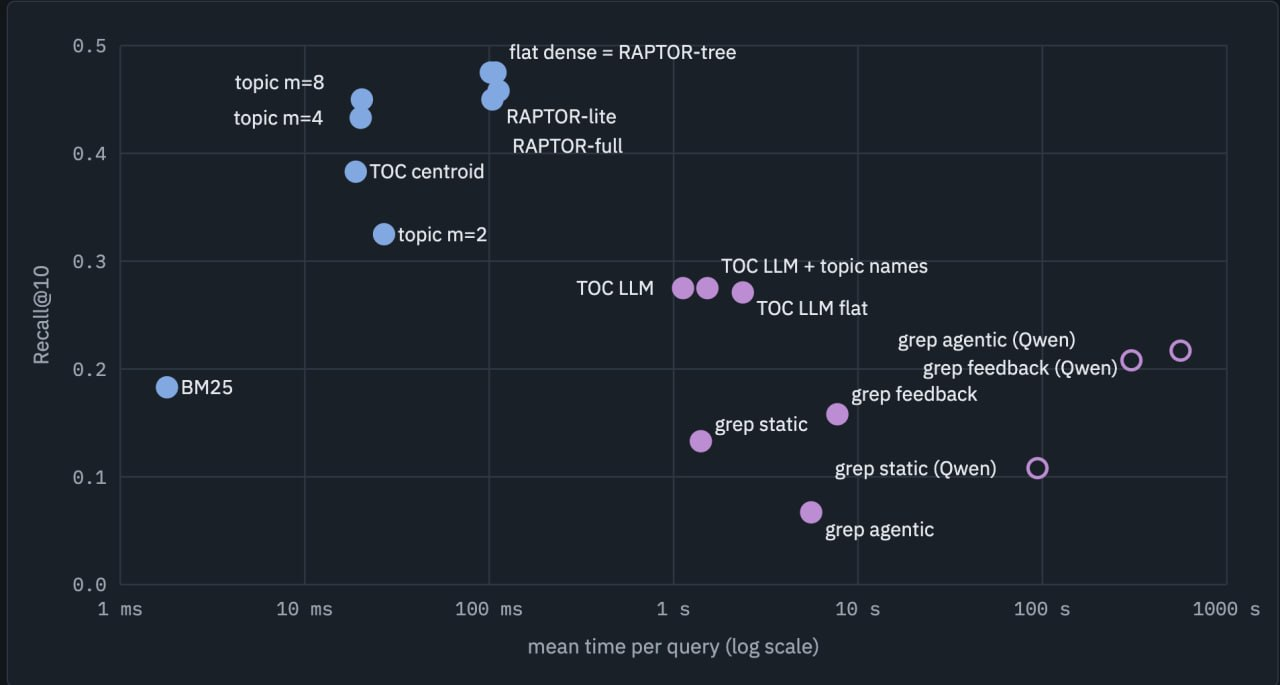
\includegraphics[width=0.6\linewidth]{images/retrieval-time-per-query.jpg}
\caption{Recall@10 against mean retrieval time per query (log scale) for the methods we tried. Blue methods make no LLM call at query time. Purple methods call an LLM: filled markers use Llama~3.3, and hollow markers use Qwen with its reasoning. Up and to the left is better. \textcolor{red}{TODO: it should not be a screenshot}}
\label{fig:speed-quality}
\end{figure}

Figure~\ref{fig:speed-quality} places every method we tried by quality and retrieval time; up and to the left is better. Flat dense search and the summary trees sit together at the top, at about 100\,ms per question, and nothing lies beyond them. Table~\ref{tab:retrieval} gives NDCG@10 on dev for the methods that ran on the full splits.
\\
The cheapest methods match strings rather than meaning. BM25 answers in about 2\,ms but reaches only 0.227 NDCG@10, because the forum answers rarely reuse the question's words. String methods could still compete in a system that learns from its users over time, as web search learns from clicks~\citep{joachims2002clickthrough}, but our task offers no such feedback.
\\
Grep was our test of whether a modern LLM could make up for this. \citet{sen2026grep} found that grep beats vector search for agents working over conversation history, but here it did not. The best variant reached a Recall@10 of about 0.22, against 0.48 for dense search, and took seconds to minutes per question. A regular expression finds words, while our questions need records that share meaning. Letting Qwen reason before writing patterns~\citep{wei2022cot} helped one variant and hurt another while adding 70--100\,s per call, so we dropped it. Grep suits searches where exact tokens matter, such as identifiers in code, and lexical methods remain an option where a vector index is impossible. Here, though, they are no substitute for one.
\\
Routing and graphs lose quality for little gain. Searching only the 8 nearest of 256 topics, 3\% of the corpus, costs 0.021 NDCG@10. An LLM reading a table of contents routes worse than plain centroids. Both graphs scored well below dense search even on a 600-record subset: 0.387 and 0.472, against 0.790.


% Figure~\ref{fig:speed-quality} maps every method we tried, and Table~\ref{tab:retrieval} gives NDCG@10 on dev. Flat dense search and the summary trees share the top of the chart at about 100\,ms, and no method lies above and to the left of them.

% \paragraph{String matching is fast but blind to meaning.} BM25 answers in about 2\,ms but reaches only 0.227 NDCG@10. The records are paraphrase-heavy forum answers, and matching strings misses that two phrasings mean the same thing. Such methods could still compete if the system learned what users find relevant over time, as search engines learn from clicks~\citep{joachims2002clickthrough}. In a feedback-driven system they might even beat dense RAG. Our task has no feedback signal, so we did not pursue them.
% \vspace{-0.7em}
% \paragraph{Grep: an agent does not make up for missing semantics.} \citet{sen2026grep} report that grep beats vector retrieval for agents searching conversation history, so we tested whether a modern LLM could make grep work here too. It could not: the best variant reached only about 0.22 Recall@10, against 0.479 for dense search. Grep matches strings, but our answers share meaning with the question, not words. It suits search where exact tokens matter, such as identifiers in a codebase or names in a chat log.
% \\
% We also let Qwen reason before writing patterns, a form of chain of thought~\citep{wei2022cot}. That helped agentic grep (Recall@10 0.067 to 0.208) but hurt static grep (0.133 to 0.108), and each call spent 70--100\,s on hidden reasoning, so we dropped it. These methods remain candidates where a vector index is not possible, but not as a replacement for one.
% \vspace{-0.7em}
% \paragraph{Routing and graphs.} Topic routing trades quality for search size: searching 8 of 256 topics, or 3\% of the records, costs 0.021 NDCG@10. Routing by an LLM over the TOC was slower and worse than routing by centroid. Graphs were the weakest family. On a 600-record subset, NDCG@10 was 0.387 for the LLM graph and 0.472 for the lazy graph, against 0.790 for dense search.

\begin{table}[t]
\centering
\footnotesize
\setlength{\tabcolsep}{4pt}
\begin{tabular}{llrr}
\toprule
Method & Build cost & Searched & NDCG@10 \\
\midrule
Dense baseline (\texttt{enc\_a}) & none & 100\% & 0.402 \\
RAPTOR-tree, gpt-5-mini (exp./evid.) & 272 summ., \$1.46 & 100\% & 0.401 / 0.400 \\
RAPTOR-tree, Llama~3.3 (exp.\,/\,evid.) & 439 calls, free & 100\% & 0.396 / 0.398 \\
RAPTOR-lite (exp.\,/\,evid.) & LLM summaries & 100\% & 0.399 / 0.398 \\
Faithful RAPTOR, gpt-4o-mini (exp./evid.) & 5,243 calls, \$1.11 & 100\% & 0.383 / 0.348 \\
Topic routing, $m = 8/4/2$ of 256 & CPU minutes & 3.1 / 1.6 / 0.8\% & 0.381 / 0.342 / 0.289 \\
TOC routed by centroid, $m=4$ & CPU minutes & -- & 0.302 \\
BM25 & seconds & 100\% & 0.227 \\
\bottomrule
\end{tabular}
\caption{Retrieval structures on the 125 dev questions, for methods with no LLM call at query time. The build cost is one-off, in US\$. Rerankers are in Table~\ref{tab:final}.}
\label{tab:retrieval}
\end{table}
\vspace{-0.7em}
Summary trees came closest but never beat the baseline. With free Llama summaries, RAPTOR-tree scored 0.398. Rebuilt with paid gpt-5-mini summaries, to check whether summary quality was the problem, it scored 0.400. The faithful version of the paper did worse, at 0.348--0.383: 95\% of its summaries stop mid-sentence at the 100-token cap, and its 5,243 summary nodes crowd records out of the top 10. All versions fail for the same reason. The summaries are broad topic overviews, such as lists of apps, books or rules, while each question asks for one specific answer that a single record already contains.

\subsection{A stronger ranking model is where retrieval improves}

Rerankers were the one change that moved retrieval, even though they only reorder the dense top 20 and so cannot recover the 42\% of labelled records that lie outside it. The small MiniLM made things slightly worse, at 0.393, because, trained on web search, it prefers records that repeat the question's words. Fine-tuning it on our practice labels did not help: it scored 0.466 on the questions it trained on, but 0.371 on dev. Practice and dev share no relevant records. With only 793 positive examples, the 22M-parameter model memorised which records were relevant instead of learning what makes a record relevant, and lost what it knew from MS MARCO. The two larger rerankers, by contrast, gave the clearest gains of the project. They raised NDCG@10 to 0.460 and 0.465, with intervals well clear of zero (Table~\ref{tab:final}).


\subsection{The judged answers do not follow}

\begin{table}[t]
\centering
\footnotesize
\setlength{\tabcolsep}{3pt}
\begin{tabular}{lrrlrrl}
\toprule
Method & R@5 & NDCG@10 & $\Delta$NDCG@10 [CI] & Out/in & Score & $\Delta$Score [CI] \\
\midrule
Baseline (dense) & .382 & .402 & -- & -- & .687 & -- \\
+ MiniLM & .381 & .393 & $-.008$ $[-.044, .025]$ & 18/19 & .646 & $-.041$ $[-.095, .011]$ \\
+ bge-reranker-v2-m3 & .467 & .460 & $\mathbf{+.058}$ $\mathbf{[.023, .098]}$ & 16/38 & .661 & $-.026$ $[-.082, .033]$ \\
+ mxbai-rerank-base-v2 & .470 & \textbf{.465} & $\mathbf{+.063}$ $\mathbf{[.027, .101]}$ & 10/34 & .678 & $-.009$ $[-.063, .045]$ \\
RAPTOR-tree (evidence) & -- & .400 & -- & -- & .690 & $+.003$ $[-.045, .051]$ \\
\bottomrule
\end{tabular}
\caption{Answer-level comparison on the 125 dev questions (whisper-1 transcripts, Qwen~3.5 answers, Mistral Small~4 judge, one run per method). Score $=$ (correctness $+$ grounding $+$ completeness)$/12$. $\Delta$ is the mean paired difference against the baseline with its 95\% bootstrap interval; bold intervals exclude zero. Rerankers rescore the dense top 20; out/in counts relevant records moved out of / into the top 5. R@5 is Recall@5.}
\label{tab:final}
\end{table}

We expected better retrieval to give better answers, but Table~\ref{tab:final} shows that it did not. The two larger rerankers put about twice as many relevant records into the prompt as MiniLM, yet their answer scores moved by only $-0.026$ and $-0.009$, inside the noise. Neither RAPTOR-tree nor MiniLM changed the score measurably either.
\\
RAPTOR-tree shows most clearly what is going on. A summary reached the top five in only 10 of the 125 dev questions, each time pushing out the fifth-ranked record, never a relevant one. On the other 115 questions, the prompt was exactly the baseline's, yet regenerating and re-judging those identical prompts changed the score on 58 of them. Of the 10 questions where a summary did enter the prompt, 7 scored the same as the baseline. Whatever RAPTOR changes is far smaller than the noise in a single judged run~\citep{zheng2023judging}.
\\
The judge also barely rewards retrieval itself. The baseline scores 0.681 on dev questions with no relevant record in its top five, and 0.691 on questions with one. The judge rates how well an answer uses the evidence it was given, not whether that evidence was right. A judge that cannot tell these cases apart, and that changes its verdict on half of identical prompts, is most likely the wrong model or the wrong set-up for this score, and we would like to investigate this further.
\\
More generally, LLM outputs are not deterministic. The harness around answering and judging therefore matters as much as the retriever: sampling settings, repeated generations and judgements, reference answers, and calibration against human ratings. The set-up we used, one generation and one judgement per question, does not meet that standard, and we did not find a robust form of it within this exercise.
\\
Cost shows the same thing. Retrieval takes 0.11\,s per question for the baseline and 1.40\,s with MiniLM on a laptop CPU. The Qwen answer takes about 74\,s, mostly about 2.9k tokens of hidden reasoning, so the choice of retriever barely changes end-to-end time: the medians range from 73.9 to 80.0\,s.

\subsection{Closing the loop with our own ASR}
\label{sec:asr-swap}

Passing the kernel tests shows that each operation is correct, not that the whole model is good enough for this task. We therefore compared our ASR with whisper-1 inside the full system. We transcribed the 125 dev questions with GLM-ASR-Nano on our kernels, in a 17-minute job on an NVIDIA L40S: 13 minutes went to loading the model, then each question took a median of 1.45\,s. We then reran the baseline and RAPTOR-tree with only the transcripts changed.
\\
The transcripts are not identical, but the differences are of a kind that does not change what the system does. Of the 125 transcripts, 76 are byte-identical, and 24 differ only in case or punctuation. Of the 25 that differ in words, 18 are formatting, such as ``two thousand'' for ``2000'' or ``H one B'' for ``H-1B''. Only 5 are mishearings by our model, against 2 by whisper-1.
\\
We checked several of the formatting cases by hand in the front end, and the generator understood them. In Figure~\ref{fig:h1b}, it reads ``H one B visa'' as an H-1B visa, and even cites a record on H1B tax reporting. We therefore added no text normalisation after the ASR. Retrieval moved by less than 0.005 NDCG@10. The answer score changed by $+0.002$ $[-0.034, 0.040]$ for the baseline and $-0.027$ $[-0.062, 0.009]$ for RAPTOR-tree. Our ASR can therefore replace whisper-1, a paid service, at no measurable cost to the system. Appendix~\ref{appendix:side} reports two smaller side experiments, on the encoder and the context builder.


% \vspace{-0.7em}
% \paragraph{The judging harness is the bottleneck.} We therefore do not read Table~\ref{tab:final} as ``better retrieval does not help''. A judge that barely separates answers built on relevant and irrelevant evidence, and that changes its verdict on half of identical prompts, is most likely the wrong model, or the wrong set-up, for this score; we would like to investigate this in detail. More broadly, because LLM outputs are not deterministic, the harness around both answering and judging (sampling settings, repeated generations and judgements, reference answers, calibration of the judge against human labels) matters as much as the retriever. The set-up we used, one generation and one judgement per question, does not meet that standard, and we did not find a robust form of it within this exercise; building one is the main step for future work.

% \subsection{Validating our own ASR end to end}
% \label{sec:asr-swap}

% \paragraph{Setup.} Kernel tests show that each operation is correct, but not that the whole model is good enough for the task, so we checked our ASR against whisper-1. GLM-ASR-Nano on our kernels transcribed the 125 dev questions in one 17-minute job on an NVIDIA L40S. Loading the model took 13 minutes, and transcription took a median of 1.45\,s per question. There the kernels also passed all tests (893\,ms for the test sentence). We then reran the baseline and RAPTOR-tree with only the transcript file changed (500 ELM calls, no failures).
% \vspace{-0.7em}
% \paragraph{Transcripts.} Compared with whisper-1, 76 transcripts are byte-identical, and 24 differ only in case or punctuation. Of the 25 that differ in words, 18 are formatting differences, such as ``two thousand'' for ``2000'' or ``H one B'' for ``H-1B''. Our model misheard 5 questions and whisper-1 misheard 2. We checked several of these by hand in the front end, typing each question both ways. In Figure~\ref{fig:h1b}, for example, the generator reads ``H one B visa'' as H-1B and even cites a record on H1B tax reporting. We therefore added no text normalisation after the ASR.
% \vspace{-0.7em}
% \paragraph{Retrieval and answers.} Retrieval moved by less than 0.005 NDCG@10. The score changed by $+0.002$ $[-0.034, 0.040]$ for the baseline and by $-0.027$ $[-0.062, 0.009]$ for RAPTOR-tree, so neither change is measurable. Our ASR therefore does the job as well as whisper-1, a paid model with a median of 1.13\,s per question, while ours is free and runs on our own kernels.
% \\
% Appendix~\ref{appendix:side} reports two side experiments (encoder migration and context builders).
 


\section{Discussion and Conclusion}
\label{sec:conclusion}

For spoken single-hop finance questions, flat dense retrieval is already close to the best quality available for its cost, as we expected. None of the structures we added beat it, and LLM calls at query time made retrieval slower and worse. Retrieval did improve with a stronger ranking model, and the bge-small encoder in Appendix~\ref{appendix:side} points the same way. These gains, however, did not reach the judged answers. We read this as a limit of the measurement rather than of retrieval: the judge rewards grounding in whatever evidence it is shown, and its noise is as large as the effects we compare. Our own ASR, meanwhile, matches whisper-1 wherever we measured. The study cost about US\$3 in paid API calls, under one GPU-hour on an L40S and 0.55 on an H200.
\\
The main limitation is therefore the answering and judging harness, and that is where we would go next. We would try other judge models and prompts, repeat generations and judgements, add reference answers, and check the judge against a small set of human ratings. We would then rerun the final comparison, including the larger rerankers combined with the bge-small encoder. Two further limitations apply. The labels mark only answers from each question's original forum thread, which penalises methods that find different but valid evidence. Our timings also come from a laptop CPU and a shared model, and the larger rerankers have not yet been timed.


% References are excluded from the main-body page limit.
\bibliography{references}
\bibliographystyle{iclr2027_conference}

% Put your Appendix here if needed. Comment out if you don't need it.
\appendix
% \section{Appendix title}
% Appendix here. Please notice that reviewers are not obliged to read Appendix at all. Please put your main content in the main body.

\section{Complete Homework 1 outputs}
\label{appendix:hw1-outputs}
 
All outputs below come from the same session on the GPU node.
\vspace{0.5em}
\\
Output of \texttt{nvidia-smi -L}:
\begin{lstlisting}[breaklines=true, basicstyle=\ttfamily\footnotesize]
GPU 0: NVIDIA H200 (UUID: GPU-25cb7a7a-ecd5-0631-5f9d-f4fec9d38b9c)
  MIG 3g.71gb     Device  0: (UUID: MIG-033534e4-2c01-566d-83a7-2305f2f03e86)
\end{lstlisting}
Output of \texttt{make test}:
\begin{lstlisting}[breaklines=true, basicstyle=\ttfamily\footnotesize]
nvcc -O3 -std=c++17 -lineinfo -diag-suppress 177 -arch=sm_90 -Xcompiler -fPIC -Icsrc -c csrc/task1_rope.cu -o build/sm_90/obj/task1_rope.o
nvcc -O3 -std=c++17 -lineinfo -diag-suppress 177 -arch=sm_90 -Xcompiler -fPIC -Icsrc -c csrc/task2_reduce.cu -o build/sm_90/obj/task2_reduce.o
nvcc -O3 -std=c++17 -lineinfo -diag-suppress 177 -arch=sm_90 -Xcompiler -fPIC -Icsrc -c csrc/task3_gemm.cu -o build/sm_90/obj/task3_gemm.o
nvcc -O3 -std=c++17 -lineinfo -diag-suppress 177 -arch=sm_90 -Xcompiler -fPIC -Icsrc -c csrc/task4_attention.cu -o build/sm_90/obj/task4_attention.o
nvcc -O3 -std=c++17 -lineinfo -diag-suppress 177 -arch=sm_90 -Xcompiler -fPIC -Icsrc -c csrc/provided.cu -o build/sm_90/obj/provided.o
nvcc -O3 -std=c++17 -lineinfo -diag-suppress 177 -arch=sm_90 -Xcompiler -fPIC -Icsrc -shared build/sm_90/obj/task1_rope.o build/sm_90/obj/task2_reduce.o build/sm_90/obj/task3_gemm.o build/sm_90/obj/task4_attention.o build/sm_90/obj/provided.o -o build/sm_90/libasr_kernels.so
nvcc -O3 -std=c++17 -lineinfo -diag-suppress 177 -arch=sm_90 -Xcompiler -fPIC -Icsrc tests/test_task1_rope.cu build/sm_90/obj/task1_rope.o build/sm_90/obj/task2_reduce.o build/sm_90/obj/task3_gemm.o build/sm_90/obj/task4_attention.o build/sm_90/obj/provided.o -o build/sm_90/test_task1_rope -lcublas -Xlinker -rpath -Xlinker /opt/cuda-12.8.0/lib64
nvcc -O3 -std=c++17 -lineinfo -diag-suppress 177 -arch=sm_90 -Xcompiler -fPIC -Icsrc tests/test_task2_reduce.cu build/sm_90/obj/task1_rope.o build/sm_90/obj/task2_reduce.o build/sm_90/obj/task3_gemm.o build/sm_90/obj/task4_attention.o build/sm_90/obj/provided.o -o build/sm_90/test_task2_reduce -lcublas -Xlinker -rpath -Xlinker /opt/cuda-12.8.0/lib64
nvcc -O3 -std=c++17 -lineinfo -diag-suppress 177 -arch=sm_90 -Xcompiler -fPIC -Icsrc tests/test_task3_gemm.cu build/sm_90/obj/task1_rope.o build/sm_90/obj/task2_reduce.o build/sm_90/obj/task3_gemm.o build/sm_90/obj/task4_attention.o build/sm_90/obj/provided.o -o build/sm_90/test_task3_gemm -lcublas -Xlinker -rpath -Xlinker /opt/cuda-12.8.0/lib64
nvcc -O3 -std=c++17 -lineinfo -diag-suppress 177 -arch=sm_90 -Xcompiler -fPIC -Icsrc tests/test_task4_attention.cu build/sm_90/obj/task1_rope.o build/sm_90/obj/task2_reduce.o build/sm_90/obj/task3_gemm.o build/sm_90/obj/task4_attention.o build/sm_90/obj/provided.o -o build/sm_90/test_task4_attention -lcublas -Xlinker -rpath -Xlinker /opt/cuda-12.8.0/lib64
GPU: NVIDIA H200 MIG 3g.71gb (sm_90), 60 SMs, peak memory bandwidth about 2407 GB/s

tiny (2 x 3 tokens, Hq=3, Hk=1)      PASS  max_err=1.08e-07     0.003 ms      0.6 GB/s ( 0% of peak)
odd sizes, partial rotation          PASS  max_err=1.08e-07     0.002 ms      7.1 GB/s ( 0% of peak)
audio encoder (partial, 32/64)       PASS  max_err=1.93e-07     0.014 ms   1075.0 GB/s (45% of peak)
text decoder (GQA 16/4, full)        PASS  max_err=1.64e-07     0.003 ms    407.2 GB/s (17% of peak)

Task 1 (RoPE): ALL PASS
GPU: NVIDIA H200 MIG 3g.71gb (sm_90), 60 SMs, peak memory bandwidth about 2407 GB/s

rmsnorm, one short row               PASS  max_err=8.27e-08     0.002 ms      0.1 GB/s ( 0% of peak)
rmsnorm, odd cols                    PASS  max_err=3.68e-07     0.003 ms     12.2 GB/s ( 1% of peak)
rmsnorm, text decoder                PASS  max_err=4.35e-07     0.005 ms    218.0 GB/s ( 9% of peak)
layernorm, odd cols (example)        PASS  max_err=3.91e-07     0.004 ms     10.6 GB/s ( 0% of peak)
layernorm, audio encoder             PASS  max_err=5.42e-07     0.013 ms   1156.3 GB/s (48% of peak)
softmax, one short row               PASS  max_err=9.28e-09     0.002 ms      0.0 GB/s ( 0% of peak)
softmax, odd cols                    PASS  max_err=9.75e-10     0.003 ms      7.4 GB/s ( 0% of peak)
softmax, large inputs (+-100)        PASS  max_err=2.67e-08     0.003 ms      5.5 GB/s ( 0% of peak)
softmax, all negative (-200..-150)   PASS  max_err=4.80e-09     0.003 ms      1.8 GB/s ( 0% of peak)
softmax, vocabulary row (59264)      PASS  max_err=6.97e-11     0.093 ms      5.1 GB/s ( 0% of peak)
softmax, 64 x 4096                   PASS  max_err=9.11e-10     0.007 ms    292.9 GB/s (12% of peak)

Task 2 (reductions): ALL PASS
GPU: NVIDIA H200 MIG 3g.71gb (sm_90), 60 SMs, peak memory bandwidth about 2407 GB/s

tiny 3 x 5, K = 7                    PASS  max_err=9.76e-09     0.002 ms        0 GFLOP/s
    for comparison: naive      0 GFLOP/s, cuBLAS      0 GFLOP/s (CPU reference)
odd sizes 37 x 100, K = 33, bias     PASS  max_err=1.55e-07     0.003 ms       86 GFLOP/s
    for comparison: naive     72 GFLOP/s, cuBLAS     42 GFLOP/s (CPU reference)
odd sizes, bias + GELU               PASS  max_err=7.70e-07     0.005 ms      187 GFLOP/s
    for comparison: naive    127 GFLOP/s, cuBLAS    140 GFLOP/s (CPU reference)
decoder q_proj (64x2048x2048)        PASS  max_err=1.05e-05     0.174 ms     3078 GFLOP/s
    for comparison: naive    396 GFLOP/s, cuBLAS  13949 GFLOP/s (cuBLAS reference)
decoder gate_proj (64x6144x2048)     PASS  max_err=1.14e-05     0.503 ms     3204 GFLOP/s
    for comparison: naive    407 GFLOP/s, cuBLAS  15873 GFLOP/s (cuBLAS reference)
decoder down_proj (64x2048x6144)     PASS  max_err=3.53e-05     0.569 ms     2831 GFLOP/s
    for comparison: naive    386 GFLOP/s, cuBLAS  17570 GFLOP/s (cuBLAS reference)
lm_head, last token (1x59264x2048)   PASS  max_err=1.24e-05     1.113 ms      218 GFLOP/s
    for comparison: naive    211 GFLOP/s, cuBLAS   1134 GFLOP/s (cuBLAS reference)
encoder q_proj (1500x1280x1280)      PASS  max_err=9.66e-06     1.424 ms     3453 GFLOP/s
    for comparison: naive    415 GFLOP/s, cuBLAS  20950 GFLOP/s (cuBLAS reference)
encoder fc1 + GELU (1500x5120x1280)  PASS  max_err=6.92e-07     5.604 ms     3509 GFLOP/s
    for comparison: naive    416 GFLOP/s, cuBLAS  23005 GFLOP/s (cuBLAS reference)
conv2 via im2col (1500x1280x3840)    PASS  max_err=2.74e-05     4.294 ms     3434 GFLOP/s
    for comparison: naive    416 GFLOP/s, cuBLAS  22515 GFLOP/s (cuBLAS reference)

Task 3 (tiled GEMM): ALL PASS
GPU: NVIDIA H200 MIG 3g.71gb (sm_90), 60 SMs, peak memory bandwidth about 2407 GB/s

tiny, one tile (4 queries, 5 keys)   PASS  max_err=1.11e-07     0.005 ms        1 GFLOP/s
several tiles, peaky scores          PASS  max_err=4.97e-07     0.019 ms       12 GFLOP/s
GQA 4 heads / 2 kv heads             PASS  max_err=1.30e-07     0.008 ms       75 GFLOP/s
causal, seq_q = seq_k                PASS  max_err=4.86e-07     0.031 ms       82 GFLOP/s
causal, 5 new queries, 37 keys       PASS  max_err=1.78e-07     0.010 ms       19 GFLOP/s
causal, one new query                PASS  max_err=3.39e-07     0.031 ms       19 GFLOP/s
text decoder (GQA 16/4, causal)      PASS  max_err=5.21e-07     0.029 ms      578 GFLOP/s
audio encoder (20 heads, 1500)       PASS  max_err=2.68e-07     6.302 ms     1828 GFLOP/s

Task 4 (attention): ALL PASS

\end{lstlisting}

Output of \texttt{./run.sh -{}-profile}:
\begin{lstlisting}[breaklines=true, basicstyle=\ttfamily\footnotesize]
GPU: NVIDIA H200 MIG 3g.71gb (sm_90)
Kernels: rope=cuda  reduce=cuda  gemm=cuda  attention=cuda  provided=cuda
Library: /home/s2984817/edin-mls-26-autumn/hw1-asr/build/sm_90/libasr_kernels.so
Loading the model (about 9 GB of float32 weights)...
Loaded in 86.6 s
Audio: 3.50 s, mel features (1, 128, 3000), prompt 59 tokens
  run 1:   1657.3 ms  (13 tokens)
  run 2:   1656.8 ms  (13 tokens)
  run 3:   1657.5 ms  (13 tokens)

GPU time per operation, one transcription (1720.2 ms in kernels):
  operation    runs on    calls   total ms   share
  linear       cuda        2757     1431.1   83.2%
  attention    cuda         396      274.3   15.9%
  rmsnorm      cuda         741        6.4    0.4%
  silu_mul     cuda         364        2.7    0.2%
  rope         cuda         396        2.5    0.1%
  softmax      cuda          13        1.7    0.1%
  layernorm    cuda          65        1.0    0.1%
  embedding    cuda          13        0.4    0.0%
  im2col       cuda           2        0.1    0.0%

Time: 1657.2 ms per transcription (+/- 0.3 ms), 127.5 ms per token
Peak GPU memory: 8.56 GiB
Transcription: Concord returned to its place amidst the tents.
Expected:      Concord returned to its place amidst the tents
Accuracy: 100.0%
Status: PASS
\end{lstlisting}

\section{Side experiments}
\label{appendix:side}

\paragraph{Changing the encoder.} The course also ships corpus vectors from a second encoder, \texttt{enc\_b}, which we identified as bge-small~\citep{xiao2023cpack}. Searching those vectors with gte-small queries drops dev NDCG@10 from 0.402 to 0.349. Re-encoding the queries with bge-small recovers it, at 0.413, and adding bge-small's query prefix gives 0.434. Practice agrees, at 0.437 against 0.425, though the dev interval overlaps the baseline's. A linear map from gte space to bge space, learned on the 24,000 paired records, recovers most of the loss without changing the query encoder: 0.389 with least squares and 0.363 with Procrustes.

\paragraph{Context builders.} On 20 questions, an 800-token budget raised the answer score from 0.579 to 0.650, and removing near-duplicate records raised it to 0.671. Both used 20\% fewer prompt tokens. Given the judge noise in Section~\ref{sec:results}, 20 questions cannot support these gains, so we did not carry them forward.

% \section{Interactive front end}
% \label{appendix:frontend}

% Our front end runs any configuration preset on a spoken or typed question. Under each answer it shows what ran, stage by stage with timings, followed by the retrieved evidence with scores and the full prompt (Figure~\ref{fig:frontend}). Chats are stored only in the browser. We used it to inspect individual failures, such as the ASR formatting differences in Section~\ref{sec:asr-swap} (Figure~\ref{fig:h1b}).

% \begin{figure}[h]
% \centering
% 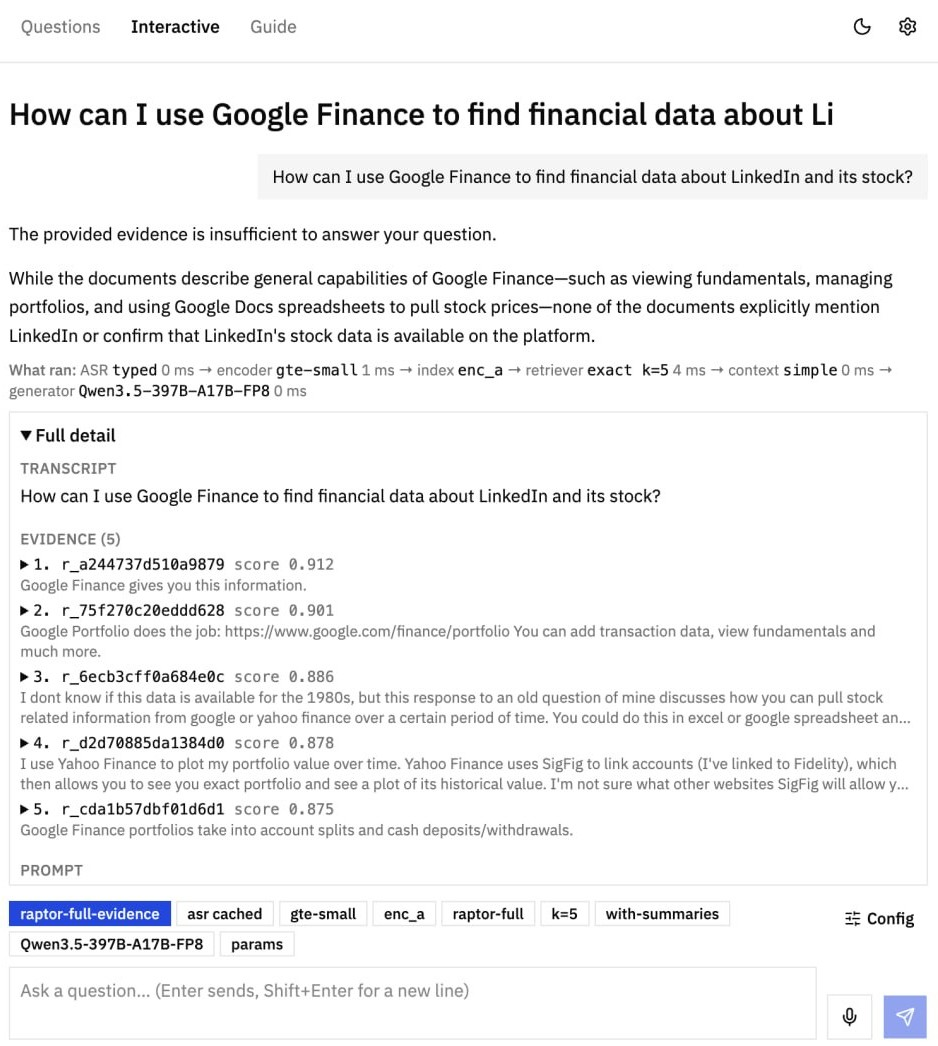
\includegraphics[width=0.8\linewidth]{images/site-trace.jpg}
% \caption{The front end answering a question with the \texttt{raptor-full-evidence} preset. The trace line lists each stage (ASR, encoder, index, retriever, context builder, generator) with its time, and the panel below shows the five retrieved records with their scores.}
% \label{fig:frontend}
% \end{figure}

% \begin{figure}[h]
% \centering
% 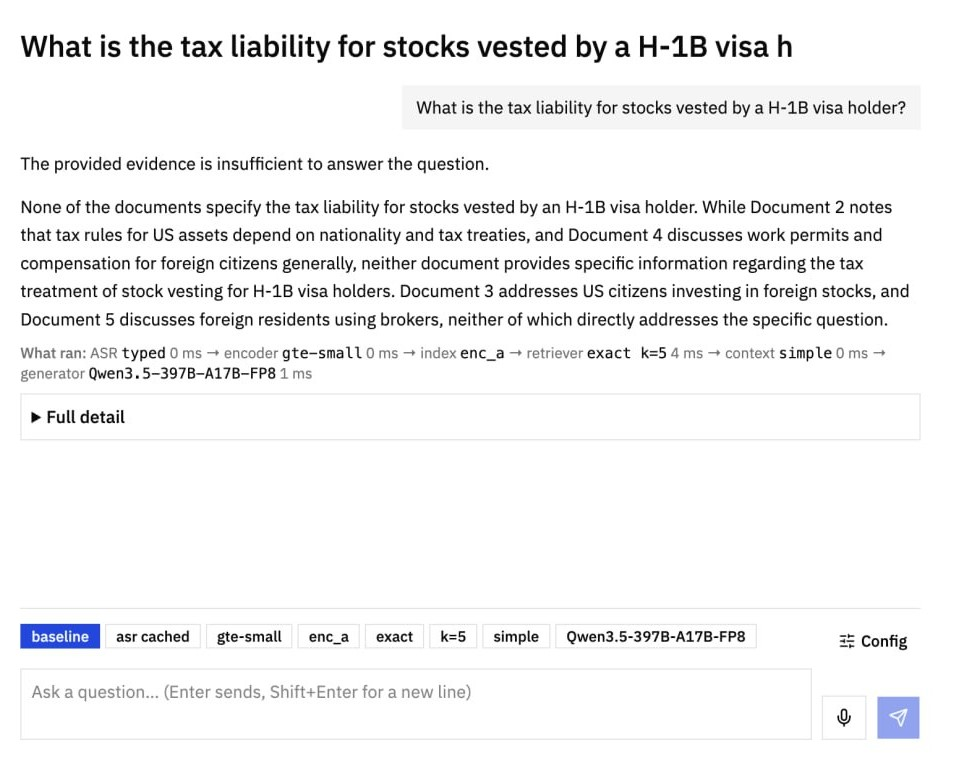
\includegraphics[width=0.49\linewidth]{images/site-h1b-typed.jpg}\hfill
% 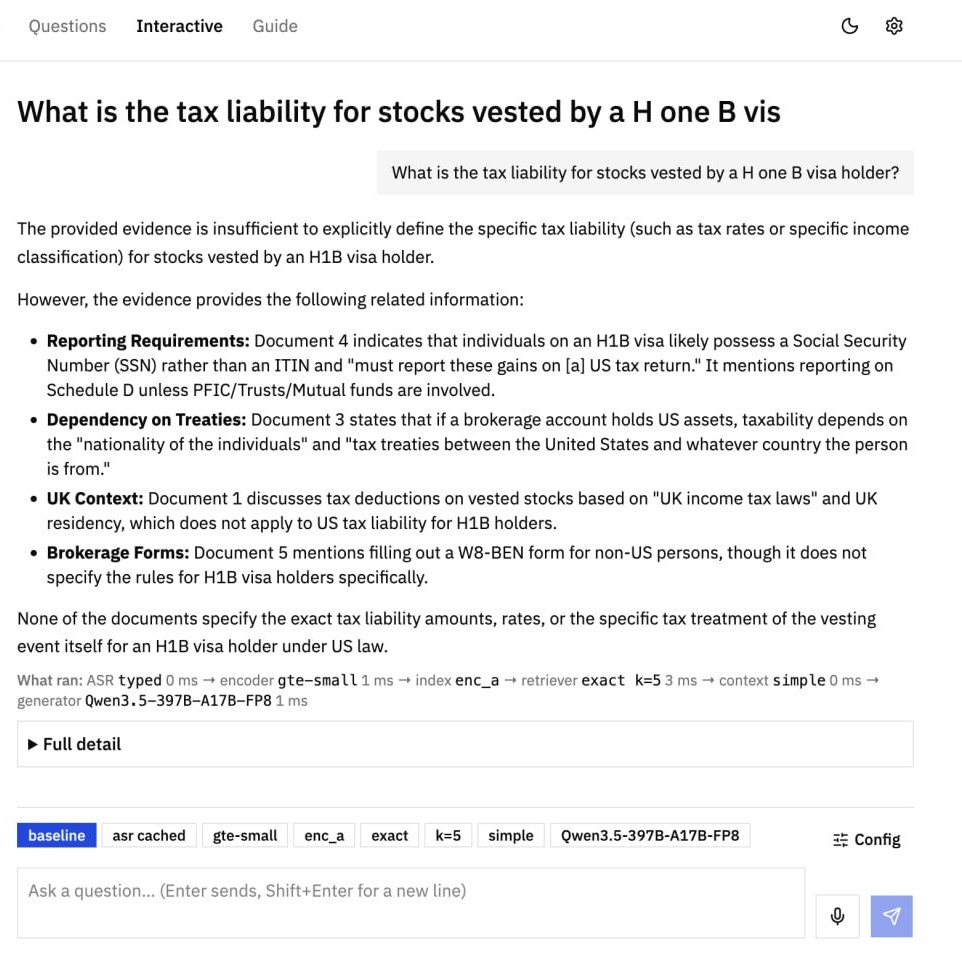
\includegraphics[width=0.49\linewidth]{images/site-h1b-spoken.jpg}
% \caption{The same question spelled as in the reference text (``H-1B'', left) and as our ASR spells it (``H one B'', right), both with the baseline preset. The generator reads ``H one B'' as H-1B, and on the right it even cites a record about H1B tax reporting. Both answers say that the evidence does not settle the exact tax liability.}
% \label{fig:h1b}
% \end{figure}

% \section{Side experiments}
% \label{appendix:side}

% \paragraph{Changing the encoder.} The course also ships corpus vectors from a second encoder, \texttt{enc\_b}, which we identified as bge-small~\citep{xiao2023cpack}. Searching those vectors with gte-small queries drops dev NDCG@10 from 0.402 to 0.349. Re-encoding the queries with bge-small recovers it, at 0.413, and adding bge-small's query prefix gives 0.434. Practice agrees, at 0.437 against 0.425, though the dev interval overlaps the baseline's. A linear map from gte space to bge space, learned on the 24,000 paired records, recovers most of the loss without changing the query encoder: 0.389 with least squares and 0.363 with Procrustes.

% \paragraph{Context builders.} On 20 questions, an 800-token budget raised the answer score from 0.579 to 0.650, and removing near-duplicate records raised it to 0.671. Both used 20\% fewer prompt tokens. Given the judge noise in Section~\ref{sec:results}, 20 questions cannot support these gains, so we did not carry them forward.

% \section{Interactive front end}
% \label{appendix:frontend}

% Our front end runs any configuration preset on a spoken or typed question. Under each answer it shows what ran, stage by stage with timings, followed by the retrieved evidence with scores and the full prompt (Figure~\ref{fig:frontend}). Chats are stored only in the browser. We used it to inspect individual failures, such as the ASR formatting differences in Section~\ref{sec:asr-swap} (Figure~\ref{fig:h1b}).

% \begin{figure}[h]
% \centering
% 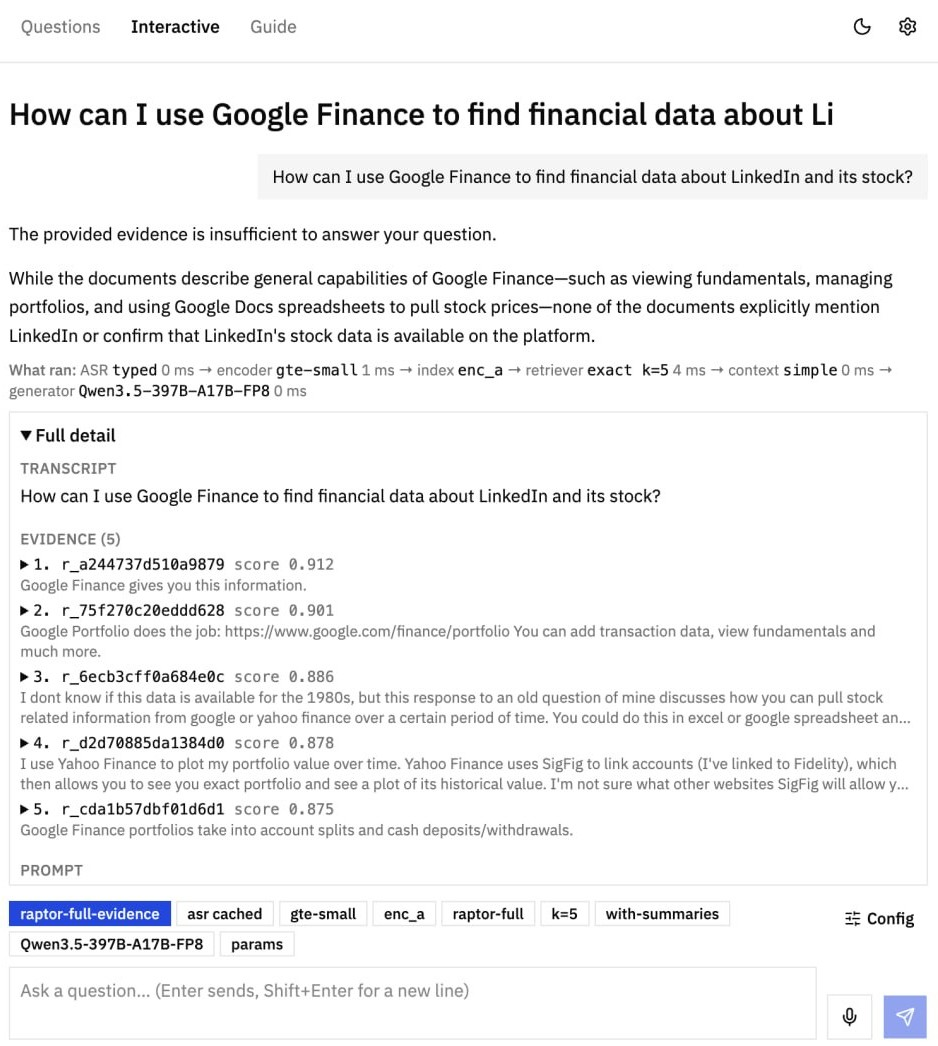
\includegraphics[width=0.6\linewidth]{images/site-trace.jpg}
% \caption{The front end answering a question with the \texttt{raptor-full-evidence} preset. The trace line lists each stage (ASR, encoder, index, retriever, context builder, generator) with its time, and the panel below shows the five retrieved records with their scores.}
% \label{fig:frontend}
% \end{figure}

% \begin{figure}[h]
% \centering
% 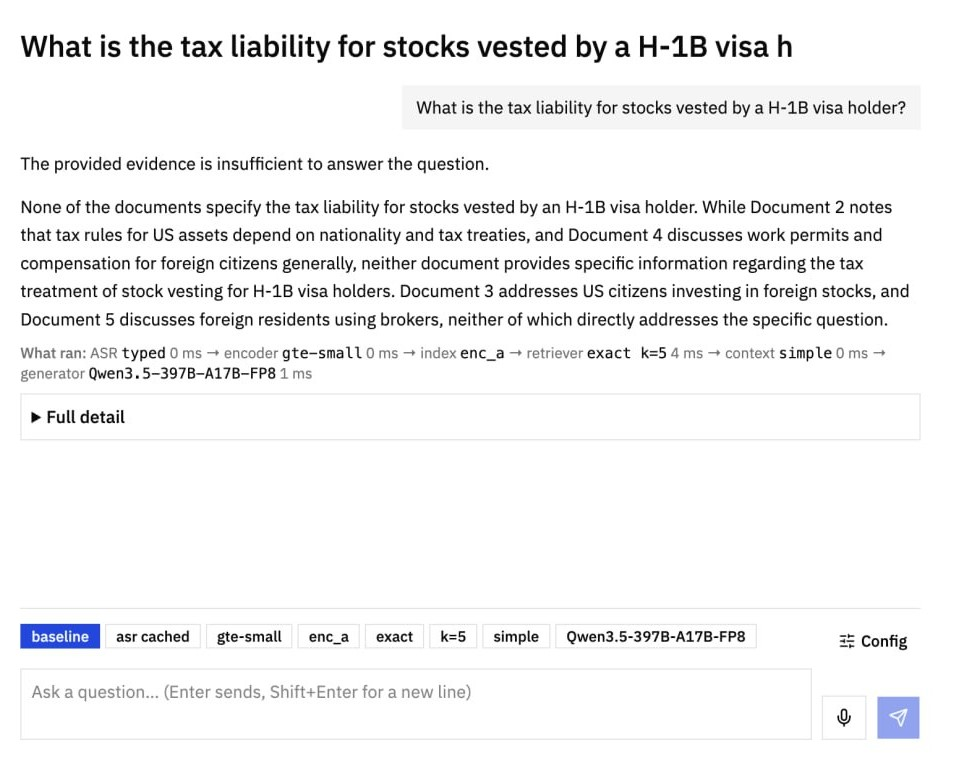
\includegraphics[width=0.5\linewidth]{images/site-h1b-typed.jpg}\hfill
% 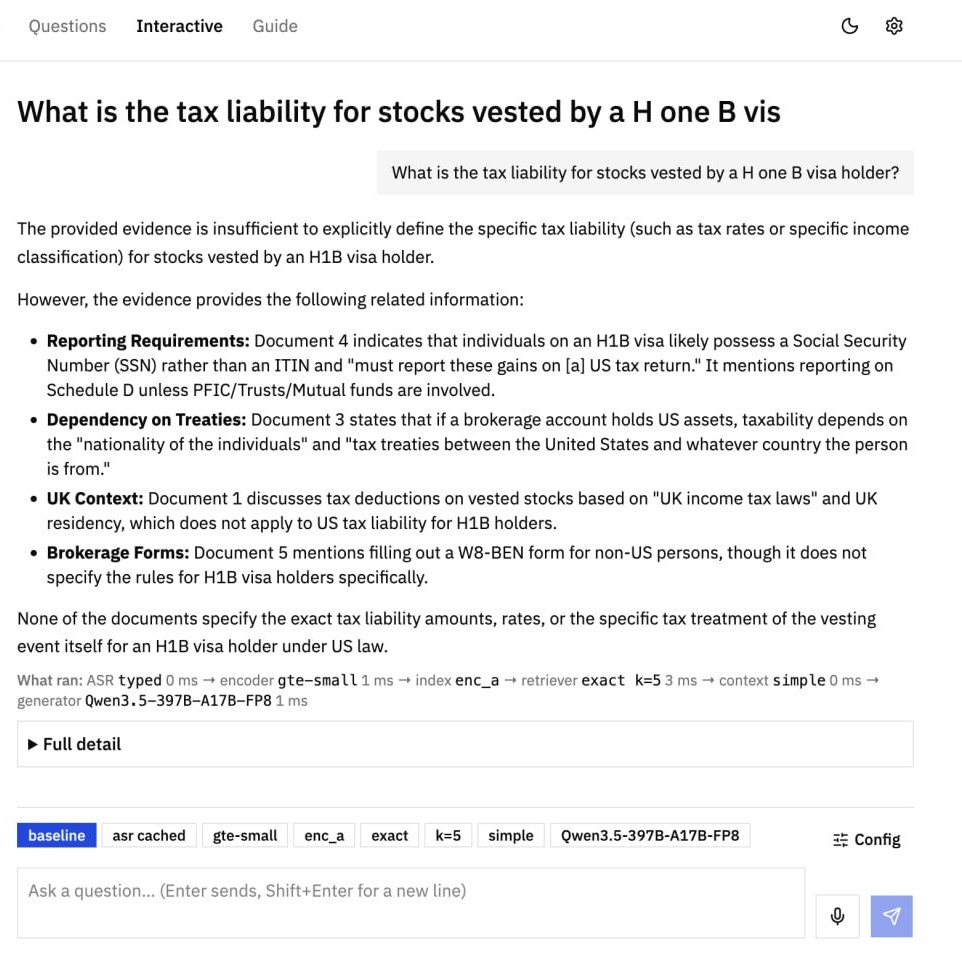
\includegraphics[width=0.5\linewidth]{images/site-h1b-spoken.jpg}
% \caption{The same question spelled as in the reference text (``H-1B'', left) and as our ASR spells it (``H one B'', right), both with the baseline preset. The generator reads ``H one B'' as H-1B, and on the right it even cites a record about H1B tax reporting. Both answers say that the evidence does not settle the exact tax liability.}
% \label{fig:h1b}
% \end{figure}



% Keep this line unchanged.
% \newpage
\clearpage


% Academic integrity is an underlying principle of research and academic practice.
% All submitted work is expected to be your own, including any material you have
% generated yourself with the assistance of AI tools such as ELM, ChatGPT,
% Bing Chat, Claude, Google Gemini, or any other automated assistance.
% For all such material you must make prominent explicit acknowledgement and
% explain clearly what you have done in this section.
% This includes using AI to directly generate text, code, figures or similar
% or to complete other tasks. In all cases, you remain entirely responsible
% for the material you produce.

\section*{AI declaration}
%Please acknowledge your use of AI here.
We used AI-based tools solely to assist with editing and improving the clarity of the manuscript text, as well as to help debug a section of our CUDA implementation and a conducting literature searches to identify related works.
\textcolor{red}{Add any other AI usage that you think we should mention}
% Please put the information of your group here without changing the format.
% This page will be deleted when the report is distributed for reviewing.
\section*{Group information}
Group ID: XXX \textcolor{red}{I'm not sure what our group ID is!}

Information of group member A:
\begin{itemize}
    \item Name: Benyamin Beyzaei
    \item UUN: s2865916
\end{itemize}
Information of group member B:
\begin{itemize}
    \item Name: Paniz Halvachi
    \item UUN: s2984817
\end{itemize}

% Keep this COMMENTED OUT, unless there is more than one member.
% Information of group member B:
% \begin{itemize}
%     \item Name: John Doe
%     \item UUN: sXXXXXXX
% \end{itemize}

% Keep this COMMENTED OUT, unless there is more than one member and you feel like
% it is necessary to point out the contribution. Please notice that members from
% the same group technically receive the same score for the report, regardless of
% the contribution.
% \section*{Contribution}


\end{document}
